\renewcommand{\encodingdefault}{OT1}
\documentclass[conference]{IEEEtran}
\IEEEoverridecommandlockouts
% The preceding line is only needed to identify funding in the first footnote. If that is unneeded, please comment it out.
\usepackage{cite}
\usepackage{amsmath,amssymb,amsfonts}
\usepackage{subcaption}
\usepackage{graphicx}
\usepackage{caption}
\usepackage{multirow}
\usepackage[Procedure]{algorithm}
%\usepackage{algorithmic}
\usepackage[noend]{algpseudocode}
\usepackage{graphicx}
\usepackage{textcomp}
\usepackage{xcolor}
\def\BibTeX{{\rm B\kern-.05em{\sc i\kern-.025em b}\kern-.08em
    T\kern-.1667em\lower.7ex\hbox{E}\kern-.125emX}}

\definecolor{orange}{rgb}{1,0.5,0}
\newcommand{\p}[1]{{\color{blue} Pdj: #1}}
\newcommand{\as}[1]{{\color{red} a: #1}}
\newcommand{\ar}[1]{{\color{red}#1}}
\usepackage{ulem}  % strike through  \sout{ }
\usepackage{url}

\usepackage{booktabs}
\begin{document}

\title{Robust Ranking of Linear Algebra Algorithms via Relative Performance\\
%{\footnotesize \textsuperscript{*}Note: Sub-titles are not captured in Xplore and
%should not be used}
\thanks{Identify applicable funding agency here. If none, delete this.}
}

\author{\IEEEauthorblockN{Aravind Sankaran}
\IEEEauthorblockA{\textit{AICES} \\
\textit{RWTH Aachen University}\\
Aachen, Germany \\
aravind.sankaran@rwth-aachen.de}
%\and
% \IEEEauthorblockN{Christos Psarras}
%\IEEEauthorblockA{\textit{AICES} \\
%	\textit{RWTH Aachen University}\\
%	Aachen, Germany \\
%psarras@aices.rwth-aachen.de}
\and
\IEEEauthorblockN{Paolo Bientinesi}
\IEEEauthorblockA{\textit{Department of Computer Science} \\
\textit{Ume\r{a} Universitet}\\
Ume\r{a}, Sweden \\
pauldj@cs.umu.se}
%\and
%\IEEEauthorblockN{4\textsuperscript{th} Given Name Surname}
%\IEEEauthorblockA{\textit{dept. name of organization (of Aff.)} \\
%\textit{name of organization (of Aff.)}\\
%City, Country \\
%email address or ORCID}
%\and
%\IEEEauthorblockN{5\textsuperscript{th} Given Name Surname}
%\IEEEauthorblockA{\textit{dept. name of organization (of Aff.)} \\
%\textit{name of organization (of Aff.)}\\
%City, Country \\
%email address or ORCID}
%\and
%\IEEEauthorblockN{6\textsuperscript{th} Given Name Surname}
%\IEEEauthorblockA{\textit{dept. name of organization (of Aff.)} \\
%\textit{name of organization (of Aff.)}\\
%City, Country \\
%email address or ORCID}
}

\maketitle

\begin{abstract}

  For a given linear algebra problem, we consider those Solution algorithms that are mathematically equivalent to one
  another, and that mostly consist of a sequence of calls to kernels from optimized libraries such as BLAS and
  LAPACK. Although equivalent (at least in exact precision), those algorithms typically exhibit significant differences
  in terms of performance, and naturally, we are interested in finding the fastest one(s). In practice, we often observe
  that multiple algorithms yield comparable performance characteristics. Therefore, we aim to identify the subset of algorithms that are reliably faster than the rest. To this end, instead of quantifying the performance of an
  algorithm in absolute terms, we present a measurement-based approach that assigns a relative score to the algorithms
  in comparison to one another. The relative performance is encoded by sorting the algorithms based on pair-wise
  comparisons and ranking them into equivalence classes, where more than one algorithm can obtain the same rank. We show
  that the relative performance leads to reliable identification of the fastest algorithms even with noisy system
  conditions.
%  Furthermore, in comparison to other metrics that quantify the performance of an algorithm in absolute
%  terms, we show that with relative performance, the fastest algorithms can be identified with fewer measurements.
  \\[4mm]


\end{abstract}

\begin{IEEEkeywords}
\textbf{performance modelling, benchmarking, sampling}
\end{IEEEkeywords}

%\p{
%  \begin{enumerate}
%  \item The conference is PMBS, not PMBC
%  \item Christos as co-author if we include MTTKRP, otherwise not.
%  \end{enumerate}
%}

\section{Introduction}

%\p{you are on top of all of this, aren't you?
%  \url{https://www.dcs.warwick.ac.uk/pmbs/pmbs/PMBS/Submit.html}
%}

Given a set $\mathcal{A}$ of mathematically equivalent linear algebra algorithms, we aim to identify the subset
$\mathcal{F} \subseteq \mathcal{A}$ containing all those algorithms that are ``equivalently'' fast to one another, and
``noticeably'' faster than any algorithm in the subset $\mathcal{A}/\mathcal{F}$. We clarify the meaning of ``equivalent'' and
``noticeable'' later in this section; for now, we simply state that in order to identify $\mathcal{F}$, 
we develop an approach that assigns a higher score to the algorithms in
$\mathcal{F}$ compared to those in $\mathcal{A}/\mathcal{F}$. Instead of aiming for a value that captures the quality of an algorithm in absolute terms, we seek to compute a relative score that compares the current algorithm with respect to the fastest algorithm(s) in $\mathcal{A}$. We refer to such scores as ``relative performance estimates''.

It is well known that execution times are influenced by many factors, and that repeated measurements, even with same input data and same cache conditions, often result in different execution times\cite{peise2014cache} \cite{hoefler2010characterizing} \cite{peise2012performance}. Therefore, finding the best algorithm is a task that involves comparing distributions of execution time.
%
In common practice, time measurements are summarized into statistical estimates (such as minimum or median execution time), which are then used to compare algorithms\cite{peise2019elaps}. \ar{But when system noise begins to have significant impact on program execution, it becomes difficult to summarize the performance into a single number; as a consequence, the comparisons are not consistent when the time measurements are reproduced, and this leads to inconsistency in the ranking of algorithms.}
% In this paper, instead of aiming for accurate estimation of distribution statistics for individual algorithms and then comparing them, we attempt to compute scores which indicate relative distance (in terms of performance) between the algorithms in $\mathcal{A}$.
%The required number of measurements also increases linearly with the number of algorithms in $\mathcal{A}$.
In order for one algorithm to be better (or worse) than the other, there should be ``noticeable`` difference in their distributions (Figure \ref{fig:diff}). On the other hand, the performance of algorithms are comparable if their distributions are ``equivalent`` or have significant overlap (Figure \ref{fig:eq}). 
%
Therefore, the result of comparing two algorithms can fall into one of the three categories - better, worse or equivalent. 
%
%The recommended approach is to find out if there is significant difference in the two distributions and eliminate the possibility of two algorithms being equivalent[hoefler]
%
\ar{In this paper, we use this three-way comparison to cluster the set of algorithms $\mathcal{A}$ into performance classes and construct a ranking that is consistent (or robust) despite noisy system conditions.} 
%
\begin{figure}[h!]
	\centering
		\begin{subfigure}[b]{0.5\textwidth}
		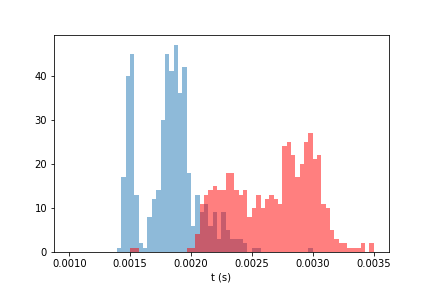
\includegraphics[width=1\linewidth]{fig/dif.png}
		\caption{Algorithms having noticeable difference in distributions}
		\label{fig:diff} 
	\end{subfigure}

	\begin{subfigure}[b]{0.5\textwidth}
		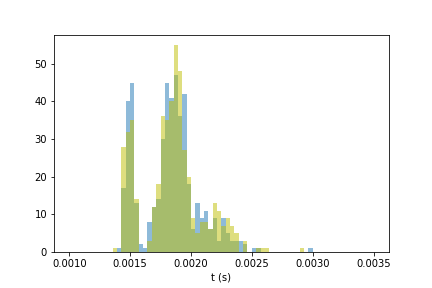
\includegraphics[width=1\linewidth]{fig/eq.png}
		\caption{Algorithms having significant overlap of distributions}
		\label{fig:eq}
	\end{subfigure}
	
	\caption{Five hundred measurements of three solution algorithms (Yellow, Blue, Red) for the Ordinary Least Square Problem}
	\label{fig:1}
\end{figure}

The algorithms in $\mathcal{A}$ represent different, alternative ways of computing the same mathematical expression. In exact arithmetic, they would all return the same quantity.  For instance,  in the expression $y_k := H^{T}y + (I_n - H^{T}H)x_k$, which appears in an image restoration application\cite{tirer2018image}, if the product $H^TH$ is computed explicitly, the code would perform a $\mathcal{O}(n^3)$ matrix-matrix multiplication; by contrast, by applying distributivity, one can rewrite this assignment as $y_k := H^{T}(y - Hx_k) + x_k$, obtaining an alternate algorithm which computes the same expression by only matrix-vector multiplications of cost $\mathcal{O}(n^2)$\footnote{Distributivity does not always lead to lower FLOP count.}. In this example, the two algorithms differ in terms of number of floating point operations (FLOPs), hence noticeable difference in terms of execution times are naturally expected. However, two algorithms may differ significantly in execution times even if they perform the same number of FLOPs, and it is even possible that higher FLOP count result in faster executions\cite{barthels2019linnea}.

%As mentioned earlier, to determine which of two algorithms is the fastest, their distributions of execution times should be compared.  The result will depend on the specific sizes of input matrices (operand sizes). Figure [1] shows the distributions of the two algorithms for image restoration for two different dimensions of $H$. When $H$ is small, both the algorithms are equally fast and we want to assign them both to $\mathcal{F}$. If the dimension of $H$ is large, the gains of distributivity starts showing and now only the second algorithm should be in $\mathcal{F}$. 

In practice, many more than two algorithms have to be considered.  For instance, for the generalized least square problem $y := (X^TS^{-1}X)^{-1}X^{T}S^{-1}z$, it is possible to find more than 100 different algorithms\footnote{reference to github repo containing the julia code} that compute the solution and that differ not more than 1.4x in terms of FLOP count.  
%the product $H^{T}H$ could be computed both by the kernel $gemm$, which implements matrix matrix multiplications, and by calling a different kernel $syrk$, which instead computes a symmetric rank-k update.
All these different algorithms arise by considering properties of input matrices (such as symmetric positive definite, lower or upper triangular etc.), different paranthesizations for matrix chains, identifying common sub-expressions, etc \cite{psarras2019linear}. In this work, we consider solution algorithms generated by the Linnea framework \cite{barthels2019linnea}. For a given mathematical expression with fixed operand size, Linnea generates a family of algorithms (in the form of Julia code \cite{julia}) consisting of (mostly but not limited to) sequences of BLAS or LAPACK calls.

\textbf{\textit{Contribution:} }The efficient computation of mathematical expressions is critical not only for complex
simulations but also for time-critical computations done on resource-constrained hardware \cite{towardsEdgeComputing}
(e.g., instantaneous object detection for autonomous driving applications \cite{connectedvehicles}). A framework that
chooses the best algorithm should take into consideration at-least the systematic noise factors, such as  regular
interrupts, impacts of  other applications that are simultaneously sharing the resources etc. Moreover, we observed that
multiple algorithms can yield similar performance profiles. Therefore,  we develop a methodology for robust identification of not one, but a set of  fast algorithms for a given operational setting. To this end, we use the bootstrapping technique\cite{bootstrap} to rank the set of equivalent algorithms $\mathcal{A}$ into clusters, where more than one algorithm can obtain the same rank.

\textit{\textbf{Organization}}: In Section \ref{sec:rel}, we highlight the challenges and survey the state of art. In section \ref{sec:torel},  we introduce the idea behind relative performance. In section \ref{sec:met}, we describe our methodology to obtain the relative scores. In section \ref{sec:exp}, we explain the effects of parameters (that are introduced as a part of our framework) and evaluate our methodology. In section \ref{sec:app}, we discuss how this research fits in a bigger picture. Finally, in section \ref{sec:con}, we  summarize with some interesting applications and discuss the need for relative performance "modelling". 
  
% We ran our experiments on ... 24 cores. To simulate system noise, we randomly switch the number of threads between 20 - 24.
%\as{TODO (finish setup)  -- (contributions) -- (organization) I ll get back here after writing the related works and experiment section }

%In this paper, we first describe the bootstrapping strategy, and show how it can be used to cluster the algorithms into equivalence classes, which encodes the relative performance. We show that, under prominent operational noise, this method can be used to get consistent estimates even with smaller sample sizes. We then use these clusters of equivalence classes for different operand sizes as ground truths to train a neural network for generalized matrix chain expressions on a fairly small training budget. We report the accuracy and precision of the predicted set of fast algorithms.
%

\section{Related Works}
\label{sec:rel}

The efficient computation of linear algebra expressions is essential as those are at the heart of a myriad of
applications in both scientific computing and data science. Users rely more and more on high-level languages and
environments such as Julia\cite{julia}, Matlab\cite{MatlabOTB}, and Tensorflow\cite{tensorflow}, which accept linear
algebra expressions as input, and internally map them to a sequence of calls to kernels from optimized libraries such as
BLAS and LAPACK. This is precisely the type of algorithms we consider in this work. The problem of mapping a target
expression to sequences of library calls is known as the Linear Algebra Mapping Problem (LAMP)\cite{psarras2019linear};
any problem instance has many mathematically equivalent solutions, and these languages have to select the best
one. However, it has been shown that most of them choose algorithms that are sub-optimal in terms of performance\cite{psarras2019linear}.


%\p{nothing wrong with this paragraph, but it does not build much of a story. Somewhere, somehow, you have to give the
%  reader a broader perspective: One way of ranking different algorithms is by predicting the performance of each of
%  them. Then, what approaches have been used in the past to predict the performance of linear algebra algorithms? Here
%  are some:
%  \begin{itemize}
%  \item FLOP count, pure and simple.
%  \item Analytical performance models with limited or without any execution of the algorithms (Roman, others).
%  \item Interpolation models: the algorithms are sampled and fitted to known/unknown models (Felix, ...).
%  \item Hierarchical approaches: the algorithms are NOT sampled, but their building blocks are (Elmar, ...). 
%  \item ...
%  \end{itemize}
%  This organization has to emerge in this section.
%}

The set of equivalent algorithms are ranked in order to identify the best candidate. One way of ranking different algorithms is by predicting the performance of each of them. The most common performance metric for linear algebra computations is the FLOP count. But FLOPs are not always direct indicators of the fastest code\cite{barthels2019linnea}. Iakymchuk et al. model the performance analytically based on FLOPs and memory access patterns\cite{iakymchuk2012modeling} \cite{iakymchuk2011execution}; while their models can represent program execution almost accurately, constructing them not only needs a deep understanding of the processor architecture, but also a detailed analysis of kernel implementations, which are not easily available.

An ideal performance metric, which should reflect the execution time of the program, would still lack in reproducibility; this is because of system noise \cite{hoefler2010characterizing}, cache effects\cite{peise2014cache}, behaviour of
collective communications \cite{agarwal2005impact}, and several other factors. Many authors have noted the lack of
textbook statistical behaviours in execution times, and it is not realistic to eliminate entirely performance variations \cite{robustbenchmarking} \cite{trackingPerfVariation} \cite{statiscalperfCompare}. 

Calotoiu et al. in \cite{calotoiu2013} use semi-analytical models, which are designed based on the understanding of computer programs behaviour in practical scenarios. Time measurements are used to determine coefficients of their models. But their focus is mainly on modelling scalability of a specific algorithm and not on identifying the best among several alternatives for a given number of processors. Our relative estimates does not capture the speed up of one algorithm over the other, but separates the fastest algorithm(s) from the rest for a given operational setting.
% without an accurate assessment of its(their) performance.

The problem we are tackling was also considered by Peise et al. in \cite{peise2012performance} but with a different approach. They model the performance (which is purely measurement-based) of BLAS calls that form the building blocks of a linear algebra program and then hierarchically compose them to predict statistical estimates of execution time for an entire algorithm. These estimates are then used to rank different variants of algorithms. However, they do not attempt to detect if two algorithms are equivalent and hence their rankings can be inconsistent (non-robust) with repeated measurements. In our work, we do not attempt to predict performance, but aim to make the performance metric more interpretable  and robust by capturing equivalence of two algorithms.  

%The measurements are repeated until the variance in execution time stabilizes. 
%
%\p{more narrative needed. Here you have the opportunity of saying that ``The problem we are tackling was also considered
%  by Peise ...'' with a different approach. Then explain differences (which you do).}  
%Peise et al in \cite{peise2012performance} use performance models to predict statistical estimates of execution time,
%which are then used to rank different variants of algorithms. However, they do not attempt to detect if two algorithms
%are equivalent and hence their predictions can be unreliable. \p{expand the concept of ``unreliable'' -- you mean that
%  if repeated twice, the process might lead to different rankings (?). You should also contrast with our title, which
%  talks about ``robust''. What do we mean by that?}
%In our work, we do not attempt to predict performance, but aim to arrive at a reliable performance metric that can
%capture equivalence of two algorithms. In a nutshell, we aim to separate the fastest algorithm(s) from the rest, without
%an accurate assessment of its(their) performance.
%
%\p{again, narrative: how does this paragraph fit the whole story? It's probably enough to flip the sentence a bit:
%``The problem of deciding whether or not two algs are equivalent performance-wise was tackled by ...''}
Guidelines for interpretable benchmarking using statistical approaches are discussed by Hoefler et al. in \cite{hoefler2015scientific}. They recommend to compute confidence intervals or conduct tests for significant differences to find out if two
algorithms are equivalent. But their focus is mainly on arriving at (absolute) performance estimates for an algorithm in isolation, whose interpretability depends on the number of measurements (sample size) used to compute such estimates. Ritter et al in \cite{ritter2020learning} proposed cost effective sampling strategies to build performance models, but again their focus is on identifying scalability bugs. On the other hand, we aim to compute interpretable "relative" estimates of algorithms in comparison to one and other, which are not influenced much by sample size (see Section \ref{sec:exp} B).
 
% Ritter et al in \cite{ritter2020learning} proposed cost effective sampling strategies to build performance models to
% help with identifying scalability bugs. By contrast, our relative estimates does not capture the speed up of one
% algorithm over the other. \p{we don't?} We assume that the basic kernel building blocks for linear algebra operations
% are already optimized for a given architecture. \p{I do not understand how this last sentence fits in the paragraph/story}
%
% \p{once again, what's the story here? how does this paragraph connect to the rest?}
% While some authors make assumptions about the that the distribution of execution time follows a normal distribution, \cite{outlierremoval} \cite{androbench} propose removal of outlier measurements for the sake of using statistical analysis designed for normal distribution. However, the true distribution of an algorithm need not necessarily follow a normal distribution on all architectures. Therefore, in this work, we do not make any assumption about the underlying distribution. 
 

%  However, instead of aiming at statistical estimates of performance (such as minimum or median execution time) for an algorithm in isolation (mainly done for scalability analysis \cite{compareEvalLinearAlg}\cite{peise2019elaps}\cite{peise2012performance}), we seek to quantify the performance relative to other algorithms in comparison. 

 %automatically map a linear algebra expression to sequence of calls to kernels from optimized libraries such as BLAS [ ] and LAPACK [ ]. They all generate 


%Common performance metrics, like those obtained by accumulating the number of arithmetic operations(FLOPs), are not always direct indicators of the fastest code; almost all high-level languages for matrix computations that map computations internally to optimized kernels such as those provided by BLAS and LAPACK, find programs that are suboptimal in terms of performance\cite{psarras2019linear}. Moreover, the prediction of performance based on FLOPs or memory-stalls, not only requires a deep understanding of the processor architecture but also a detailed analysis of kernel implementations \cite{iakymchuk2012modeling} \cite{iakymchuk2011execution}, which are not always available. An ideal performance metric, which should reflect the execution time of the program, are not exactly reproducible; this is because of system noise \cite{hoefler2010characterizing}, cache effects\cite{peise2014cache}, collective communications calls within the application\cite{agarwal2005impact} etc. Guidelines for interpretable benchmarking using statistical approaches are discussed in\cite{hoefler2015scientific}. However, instead of aiming at statistical estimates of performance (such as minimum or median execution time) for an algorithm in isolation (mainly done for scalability analysis \cite{compareEvalLinearAlg}\cite{peise2019elaps}\cite{peise2012performance}), we seek to quantify the performance relative to other algorithms in comparison. 

%Execution time … statistical approaches … drawbacks … confidence intervals … 


 
%In order to address the high computational demands With the raising number of intelligent applications (e.g., augmented reality and face recognition) that not only require much more computational power,

\section{Towards Relative Performance}
\label{sec:torel}
%The ranking methodology described in section 2 establishes a notion of distance (in terms of performance) between the algorithms in $\mathcal{A}$.
Fundamentally, we want to compute a score for every algorithm in $\mathcal{A}$ that indicates its chance of being the fastest algorithm. As an example, consider the distributions of execution times shown in Fig.~\ref{fig:1} for three different algorithms (Red, Blue and
Yellow) that solve the Ordinary Least Square problem\footnote{The pseudocode of solution algorithms are shown in Appendix A. For the sake of
  explanation, we only consider three solution algorithms; for this problem, Linnea generates many more than three,
  as explained in Sec.~4 of~\cite{barthels2019linnea}.}: $(X^TX)^{-1}X^{T}y$. 
%Since the algorithms "Red" and "Blue" are significantly overlapping, the distance between them should be less than that
%of their distances from "Green".
%\p{I think here you want to say that ``the distributions were obtained with/by the following procedure'' or something
%  like that.}
The distributions were obtained by measuring the execution time of every algorithm $\mathbf{a}_j \in \mathcal{A}$ 500 times ($|\mathbf{a}_j| = 500$).
In order to ensure that the time measurements are unbiased of system noise, we adapt the following procedure: Let the set of all executions be $\mathcal{E} = \mathbf{a}_1 \oplus \mathbf{a}_2 \oplus \mathbf{a}_3$, where $\oplus$
is a concatenation operation. The set $\mathcal{E}$ is shuffled and the executions are timed. Every execution $e \in
\mathcal{E}$ is run twice and only the second measurement is considered; the first measurement is mostly an outlier due
to loading and caching of data and instructions\cite{peise2019elaps}. 
%In practical applications, the execution times of algorithms are typically
%measured only a few times (likely fewer than 500 times, possibly just once), and therefore, only a snapshot of the distributions
%shown in Figure \ref{fig:1} will be available.
% The execution time of every algorithm $\mathbf{a} \in \mathcal{A}$ is measured $N$ times in order to get a snap shot of their respective distributions. The measured algorithms are represented as an array of size N; hence, one can also denote $\mathbf{a} \in \mathbb{R}^N$.  We do not make any assumptions about the nature of the distribution.
  %In order to understand the need to address this problem via  relative performance, we first study the limits of using absolute metrics.
A "straightforward'' approach to relatively score algorithms consists in finding the minimum (or median, or mean) execution time of every algorithm $\mathbf{a}_j \in \mathcal{A}$ and then use that to construct a ranking~\cite{peise2012performance}. By doing this, every algorithm
  would obtain a unique rank. If we choose to assign the algorithm with rank 1 to the set of fastest algorithm $\mathcal{F}$, then only one algorithm could be assigned to $\mathcal{F}$ although the distributions "Yellow" and "Blue" are nearly identical. This will lead to inconsistent rankings when all the executions $\mathcal{E}$ are repeated. Reproducibility of rankings is essential in order to derive mathematically sound performance predictions (Modelling or prediction of relative performance is a part of our future work and it is out of the scope of this article).  In order to ensure reproducibility of relative performance estimates, both "Yellow" and "Blue" should be assigned to $\mathcal{F}$. 
%  \p{ok, but what's the problem with that? since the distributions are nearly identical, there is nothing wrong in
%    selecting one over the other. I don't think this argument is valid. You want to deliver a different punchline.}
  % In such a case, only one algorithm ("Red") that has rank 1 can be reliably assigned to the set of fastest algorithms $\mathcal{F}$. 
%  \p{``consequently'' does not work here, because it's not clear where we're going.
%    Maybe ``alternatively''. But then again, I suspect we need to show different distributions to make a convincing argument}
  To this end, one could choose the $k$-best algorithms\cite{kbest-kadioglu2011algorithm} with $k=2$, and  assign both
  "Yellow" and "Blue" to $\mathcal{F}$. However, the fixed value $k=2$  might not be
  suitable for other scenarios in which either one algorithm or more than two algorithms are superior to the rest. 

  % if there is noticeable difference in the distributions between the first two algorithms, then with $k=2$, both would be assigned the same rank, which does not make sense. 
  %But there is no gaurentee that all the k-best algorithms would be equivalent for all classes of linear algebra expressions; if there is noticeable difference in the distributions between the first two algorithms, then it does not make sense to assign them with same rank. 

%\p{rephrase as: ``Bootstrapping is a common/known procedure to extract ... The idea is to ....''} 
%Alternatively, instead of relying on a single statistical estimate to construct the ranking, one could use the Bootstrapping procedure\cite{bootstrap} to obtain multiple statistics. Here, the "straightforward'' approach is repeated $T$ times, and for each iteration, $K < 500$ measurements from the original 500 measurements.


 Bootstrapping\cite{bootstrap} is a common procedure to extract more information from the distribution. Here, the "straightforward'' approach is repeated $T$ times, and for each iteration, $K < 500$ measurements are sampled from the original 500 measurements and rankings are constructed. If an algorithm $\mathbf{a_j}$ obtains rank 1 in at least one out of $T$ iterations, it is assigned to $\mathcal{F}$, and will
 receive the score of  $c/T$, where $c \le T$ is the number of times $\mathbf{a_j}$ obtains rank 1. The steps for
 this approach, adapted to our problem, are shown in Procedure \ref{alg:fa}. For a given set of algorithms $
 \mathbf{a}_1,\mathbf{a}_2 ,..., \mathbf{a}_p\in \mathcal{A}$ for which the execution times are measured $N$ times each,
 Procedure \ref{alg:fa} returns the set of fastest algorithms $f_1, f_2, ..., f_q \in  \mathcal{F}$, ($q \le p$) each with an associated score $c_1,c_2,...c_q$.
 For instance, when this procedure is applied to the distributions in Figure 1 (with $T=100$ and a sample size $K=5$ ) both "Yellow" and "Blue" are assigned to $\mathcal{F}$ with scores 0.55 and 0.45 respectively. 
%  one could repeat the "straightforward'' approach ($T$ times) on multiple samples from the original 500 measurements ($\tilde{\mathbf{a}_j} \subset \mathbf{a_j}$) and consolidate the rankings across multiple iterations; 
%\p{the concept of ``sub-sample'' is not clear} 
%This procedure is known as bootstrapping\cite{bootstrap} and 
%\p{The flow is ok, but again, it does not deliver the punchline. Here we describe the procedure, but it is not at all
%  clear if this is already a viable, conclusive solution, or if it has some kind of drawbacks. Somewhere one has to get
%  the idea that bootstrapping by itself is still lacking something.}
%For a given set of algorithms $
%\mathbf{a_1},\mathbf{a_2} ,..., \mathbf{a_P}\in \mathcal{A}$ for which the execution times are measured $N$ times each,
%Procedure \ref{alg:fa} returns the set of fastest algorithms $\mathcal{F}$, each with an associated score 
%\p{the  score will be $c_i$, right?}. 
%As mentioned, the procedure unfolds over $T$ iterations.

 
%one could use test for significant differences (such as Kruskal-Walis ANOVA[hoefler]) between algorithm pairs and merge the ranks of algorithms if there is significant overlap.

\begin{algorithm}
	\caption{ Get$\mathcal{F}$$(\mathcal{A})$ }
	\label{alg:fa}
	\hspace*{\algorithmicindent} \textbf{Input: } $ \mathbf{a}_1,\mathbf{a}_2 ,..., \mathbf{a}_p\in \mathcal{A}$ \\
	\hspace*{\algorithmicindent} \textbf{Output: } $ (f_1,c_1), (f_2, c_2), ..., (f_q,c_q) \in \mathcal{F} \times C  $
	\begin{algorithmic}[1] 
		\State $L, C \leftarrow [ \quad ]$ \Comment{Initialize empty lists}
		\For{i = 1, ..., $T$}
		\State sample $K$ values $\mathbf{\tilde{a}_{j}} \subset \mathbf{a_j} \quad \forall j$ \Comment{$ j \in \{1,..,p\}$} 
		\State append($\text{argmin}_j(\min(\mathbf{\tilde{a}}_j ), L)$ 
%		\State append($\tilde{\mathcal{F}},L$)
		\EndFor
		\State $\mathcal{F} \leftarrow $ unique elements in $L$ \Comment{ $q = |\mathcal{F}| $}
		\For{$i$ in  $f_1,f_2,...,f_q \in \mathcal{F}$}
		\State $c \leftarrow$ number of occurrences of $i$ in $L$ 
		\State append($c/T, C$)
		\EndFor
		\State return $(\mathcal{F} \times C)$
        \end{algorithmic}
%        \p{the font for T is different here and in the text}
%        \p{do not use the syntax "C.append", or "L.append"; instead: append(c/T, C), ...}
%        \p{why [ ] instead of ( ) ? argmin$( blah ) $}
%        \p{in Let, use the different direction for the assignment:
%          Instead of "Let $|\mathcal{F}| = Q$", use Let $Q = |\mathcal{F}|$. Also, $Q$ seems to be a set. Use a small
%          letter for an integer}
%        \p{I don't see the need for "$\forall j$", given that $j$ is already in "argmin"}
%        \p{rewrite the second for loop with $i$ as the index, as opposed to $f_q$}        
\end{algorithm}

%Let $\mathcal{A}(x)$ be the set of all solution algorithms for certain linear algebra expression $x$. 
However, in practical applications, the execution times of algorithms are typically
measured only a few times (likely fewer than 500 times, possibly just once), and therefore, only a snapshot of the distributions
shown in Figure \ref{fig:1} will be available. Procedure \ref{alg:fa} does not account for the uncertainty in measurement data in capturing the true distributions. 
%The scores obtained by Procedure \ref{alg:fa} still does have a meaningful translation to the indicate the distance between the algorithms; ideally, the scored obtained for "Red" and "Blue" should be comparable. This is because only one algorithm is assigned to $\mathcal{F}$ in every iteration. 
The recommended approach is to use test for significant differences (such as Kruskal-Walis
ANOVA~\cite{hoefler2015scientific}) between algorithm pairs, and to merge the ranks of algorithms if there is not enough
evidence of one algorithm dominating the other. In this paper, we incorporate the test for significant differences in
Procedure \ref{alg:fa} by re-defining the straightforward sorting function (in line 4 of Procedure 1) by introducing a
three-way comparison function. 
%As a consequence, both "Yellow" and "Blue" will be able to receive a score of 1.0.
\bigskip



\section{Methodology}
\label{sec:met}

In order to compute the relative score for an algorithm, the first step consist of sorting all the mathematically equivalent linear algebra algorithms $\mathbf{a}_1,\mathbf{a}_2, ..., \mathbf{a}_p \in \mathcal{A}$ and assigning them to one of the equivalence classes $r_1, r_2, ...r_w$. The number of classes (or ranks) is $w \le p$ as more than one algorithm can obtain the same rank. For illustration, we consider an example where four algorithms $\mathbf{a}_1,\mathbf{a}_2, \mathbf{a}_3, \mathbf{a}_4$ could be sorted and ranked as $< (\mathbf{a}_2,1), (\mathbf{a}_4,1), (\mathbf{a}_1,2), (\mathbf{a}_3,2) >$. All the algorithm with rank 1 are assigned to the set of fastest algorithms $\mathcal{F}$. The assignments of ranks need not be deterministic. So in the second step, we bootstrap and repeat this procedure $T$ times and all the algorithms that obtained rank 1 at least once are assigned to $\mathcal{F}$. Then, we follow the steps from line 5 - 9 in Procedure \ref{alg:fa} to compute relative scores. 

The execution time of every algorithm $\mathbf{a} \in \mathcal{A}$ is
measured $N$ times. The measurements are stored in an array of size N; hence, one can also denote
$\mathbf{a} \in \mathbb{R}^N$. We do not make any assumptions about the nature of the distribution. To compare the
distributions of two algorithms $\mathbf{a_i},\mathbf{a_j} \in \mathcal{A}$, we follow the steps indicated in Procedure
\ref{alg:compare}.
%\p{``method'' is not a common word for this. ``Algorithm'', ``Procedure'', ``Test'', ... Later you call it ``function'', which is also ok}
%
The comparison yields one of three outcomes:
\begin{itemize}
\item Outcome A: algorithm $\mathbf{a_i}$ is better than $\mathbf{a_j}$ $(<)$
\item Outcome B: algorithm  $\mathbf{a_i}$ is as good as $\mathbf{a_j}$ $(\sim)$
\item Outcome C: algorithm  $\mathbf{a_i}$ is worse than $\mathbf{a_j}$ $(>)$
\end{itemize}
Outcomes A and C imply that there are noticeable differences between the distributions; outcome B implies that the distributions are equivalent.
\begin{algorithm}
	\caption{Compare $(\mathbf{a_i}, \mathbf{a_j})$ }
	\label{alg:compare}
	\hspace*{\algorithmicindent} \textbf{Input: } $ \mathbf{a_i}, \mathbf{a_j} \in \mathbb{R}^{N}$ \\
	\hspace*{\algorithmicindent} \textbf{Output } $\in  \{<,>,\sim \}$
	\begin{algorithmic}[1] 
		\State $p \leftarrow 0$
		\For{i = 1, ..., $M$}
		\State sample $K$ values $\mathbf{\tilde{a}_i} \subset \mathbf{a_i}$
		\State sample $K$ values $\mathbf{\tilde{a}_j} \subset \mathbf{a_j}$
		\State $e_i$ = min($\mathbf{\tilde{a}_i}$)
		\State $e_j$ = min($\mathbf{\tilde{a}_j}$)
		\If{$e_i \le e_j$}
		\State $p=p+1$
		\EndIf
		\EndFor
		\If{$\frac{p}{M} \geq threshold$ }
		\State return $<$ \Comment{$\mathbf{a_i}$ is better than $\mathbf{a_j}$}
		\ElsIf{$\frac{p}{M} < 1 - threshold$}
		\State return $>$ \Comment{$\mathbf{a_i}$ is worse than $\mathbf{a_j}$}
		\Else
		\State return $\sim$ \Comment{$\mathbf{a_i}$ is as good as $\mathbf{a_j}$}
		\EndIf
	\end{algorithmic}
	%              \p{I don't like ``thresh'' -- either shorten it to $t$, $T$, or write it our ``threshold''.
	%                Also, here it's thresh, but in the text it's $thresh$ -- be consistent!}
      \end{algorithm}
%\p{The level of detail is good, but the connection is missing. ``To this end'' is not linking to anything.
%  Also, use references (``one could also use other metrics'' -- as done in [ref], [ref].}  
In Procedure \ref{alg:compare}, the distributions $\mathbf{a_i}$ and $\mathbf{a_j}$ are sampled ($\mathbf{\tilde{a}_i} \subset \mathbf{a_i}$ and $\mathbf{\tilde{a}_j} \subset \mathbf{a_j}$) with sample size $K < N $ and the minimum
execution time from the respective samples are compared. This procedure is repeated $M$ times. In theory, one could
also use other metrics like mean or median execution time or even combination of multiple metrics across different
comparisons. Peise et al. in \cite{peisethesis} show that minimum and median statistic are less sensitive to fluctuations in execution time for linear algebra computations.  Let $e_i$ and $e_j$ be the minimum execution time of samples  $\mathbf{\tilde{a}_i}$ and $\mathbf{\tilde{a}_j}$ respectively. The probability that $e_i$ is less than $e_j$ is approximated from the results of $M$ comparisons. That is, if $e_i$ is less than $e_j$ in $p$ out of $M$ comparisons, then the empirical probability $P[e_i \le e_j]$ is $p/M$. The outcome of the Compare function (Procedure \ref{alg:compare}) is determined based on this empirical probability (see lines 9 - 14 in Procedure \ref{alg:compare}). The outcome of Compare function is not entirely deterministic; if $p/M \to threshold$, then  $\mathbf{a_i}$ is at the threshold of being better than $\mathbf{a_j}$ and the outcome can randomly switch between A ($<$) and B ($\sim$) when the Compare function is repeated (even for the same input distributions). Hence the comparisons need not be transitive;  $\mathbf{a_1} < \mathbf{a_2}$ and
$\mathbf{a_2} < \mathbf{a_3} $ does not imply $\mathbf{a_1} < \mathbf{a_3}$.

\textbf{\textit{Effect of} $K$:} As $K \to N$, the minimum estimates of samples ($e_i, e_j$) would approximate the minimum execution time ($m_i, m_j$) of the distributions $\mathbf{a_i}$ and $\mathbf{a_j}$ respectively and the comparison in line 7 of Procedure \ref{alg:compare} becomes more and more deterministic. As a consequence, $p/M \to 0 \lor 1$ and outcome B ($\sim$) becomes less and less likely. When $K=N$, outcome B becomes impossible and this invalidates the advantages of bootstrapping. When $K \to 1$, the minimum estimates of samples ($e_i, e_j$) would point to an instance of execution time ($t_i, t_j$) from the distribution. Then outcome B becomes more likely even for marginal overlap of distributions (as in Fig \ref{fig:diff}), especially when $threshold$ is high or $M$ is small.
%\p{better phrasing: ``Since (it was observed that) most distributions... , we use minimum execution time.''
%  Then introduce notation.}

%In general, when $K$ is decreased, $M$ should be proportionately increased in-order to have similar information gain from the distribution.
%From the results of $M$ comparisons, the probability that the minimum $m_A$ of algorithm \textbf{a} 
%\p{the notation is not helping! if alg is \textbf{a}, then its min should be $\min_{\textbf{a}}$ or $m_{\textbf{a}}$ or ...}
%is less than that of algorithm \textbf{b} ($m_B$) is approximated.  If
%

\textbf{\textit{Effect of }$threshold$:} Valid values of $threshold$ for Procedure \ref{alg:compare} lie in the range $[0.5,1]$. When $threshold \to 0.5$, the outcome B ($\sim$) becomes
less and less likely (and impossible for $threshold=0.5$), while for $threshold \to 1$, the conditions for outcomes A ($<$)
and C ($>$) becomes stricter and outcome B becomes more and more likely. 

The Compare function (Procedure \ref{alg:compare}) is used in Procedure \ref{alg:sort} to sort the algorithms $\mathbf{a}_1,\mathbf{a}_2, ..., \mathbf{a}_p \in \mathcal{A}$ and assign them to one of the equivalence classes $r_1, r_2, ..., r_w$.
The swapping procedure using bubble-sort\cite{bubblesort} with three-way comparisons is shown in Procedure \ref{alg:sort}.
%The outcome of the Sort function is a sequence of ordered algorithms $<\mathbf{s}_1, \mathbf{s}_2,
%... \mathbf{s}_p>$ and their corresponding ranks $ <r_1,r_2,...r_w> $.
%Eventually, every algorithm
%$\tilde{\mathbf{a}_j}$ should be ranked better or at least ranked the same as the next algorithm in sequence
%$\tilde{\mathbf{a}_{j+1}}$.
%\p{you are misplacing the tilde. It should be $\tilde{\mathbf{a}}_j$, not $\tilde{\mathbf{a}_j}$.
%  $\tilde{\mathbf{a}}_{j+1}$, not $\tilde{\mathbf{a}_{j+1}}$.}
%It should be noted that the Compare function is not transitive. That is,  $\mathbf{a_1} < \mathbf{a_2}$ and
%$\mathbf{a_2} < \mathbf{a_3} $ does not imply $\mathbf{a_1} < \mathbf{a_3}$. Hence, there is an element of randomness in
%the final rankings, which is addressed in Procedure \ref{alg:f}. \p{what do we mean by ``randomness'' here? Are you
%  maybe trying to say that the final outcome also depends on the order in which the algorithms are compared with one
%  another? (the order in which the pair-wise comparisons are performed)}
%The Consistency of comparison can then be defined as
%\begin{equation}
%\text{Consistency} = | 1-2P[m_A \le m_B] |
%\end{equation}  
%When  $P[m_A \le m_B] \to 1$, $m_A$ is consistently less than $m_B$, which implies algorithm \textbf{a }is consistently better than \textbf{b}. In contrast, when  $P[m_A \le m_B] \to 0$, algorithm \textbf{b} is consistently better than \textbf{a}. Consistency is at its least when $P[m_A \le m_B] = 0.5$. The hyper-parameter $thresh$  is the consistency threshold that affects the outcome of the Compare function. The  final outcome of the Compare function is either 
%\p{Paolo got here}
\begin{algorithm}
	\caption{Sort $(\mathcal{A})$ }
	\label{alg:sort}
	\hspace*{\algorithmicindent} \textbf{Input: } $ \mathbf{a}_1,\mathbf{a}_2,...\mathbf{a}_p \in \mathcal{A}$ \\
	\hspace*{\algorithmicindent} \textbf{Output: } $ < (\mathbf{a}_{s[1]},r_1), (\mathbf{a}_{s[2]}, r_2), ..., (\mathbf{a}_{s[p]},r_w) > $
	\begin{algorithmic}[1] 
		\State Initialize w $\leftarrow$ p
		%\State Initialize $r_1,....,r_w$ with consecutive ranks 
		\State Initialize $\mathbf{r}_j \leftarrow j \quad \forall j \in \{1,2,..,p\}$ \Comment{Alg ranks}
		\State Initialize $\mathbf{s}_j \leftarrow j \quad \forall j \in \{1,2,..,p\}$ \Comment{Alg index }
		%\State Initialize $\mathbf{a}_{s[j]} \leftarrow \mathbf{a}_j \quad \forall  j \in \{1,2,..,p\}$
		\For{i = 1, ..., p}
		\For{j = 0, ..., p-i-1}
		\State ret = Compare($\mathbf{a}_{s[j]}, \mathbf{a}_{s[j+1]}$)
		\If{$\mathbf{a}_{s[j+1]}$ is better than $\mathbf{a}_{s[j]}$}
		\State Swap $\mathbf{s}_{j}$ and $\mathbf{s}_{j+1}$ \label{lst:swap}
		\If{$r_{j+1} = r_j$} \label{lst:h1}
		\If{$r_{j-1} !=r_j$ or $j=0$}
		\State Increment ranks $r_{j+1}, ..., r_p$ by 1 \label{lst:h2}
		\EndIf
		\Else
		\If{$r_{j-1} = r_j$ and $j\ne0$} \label{lst:gg1}
		\State Decrement ranks $r_{j+1}, ..., r_p$ by 1 \label{lst:gg2}
		\EndIf
		\EndIf
		\ElsIf{$\mathbf{a}_{s[j+1]}$ is as good as $\mathbf{a}_{s[j]}$} \label{lst:ag1}
		\If{$r_{j+1} \ne r_j$}
		\State Decrement ranks $r_{j+1}, ..., r_p$ by 1 \label{lst:ag2}
		\EndIf
		\ElsIf{$\mathbf{a}_{s[j]}$ is better than $\mathbf{a}_{s[j+1]}$}
		\State Leave the ranks as it is
		\EndIf		
		\EndFor
		\EndFor
		\State return $< (\mathbf{a}_{s[1]},r_1), ..., (\mathbf{a}_{s[p]},r_w) >$
              \end{algorithmic}
\end{algorithm}
All the algorithms $\mathbf{a}_1, \mathbf{a}_2, .., \mathbf{a}_p \in \mathcal{A}$ are first initialized with consecutive ranks $r_j \leftarrow j$ (where $j \in\{1,2,..p\}$) according to the order in which they are given as input $<1,2,...,p> $. Initially, the number of equivalence classes $w$ is same as the number of algorithms $p$. As more than one algorithm can obtain the same rank, we use different index array to map to the position of algorithms in the sorted sequence $\mathcal{S} : < \mathbf{s}_1, \mathbf{s}_2, ..., \mathbf{s}_p >$. In the beginning, $s_j \leftarrow j$ and $ \mathbf{a}_{s[j]} \leftarrow \mathbf{a}_j$. Thus, Procedure \ref{alg:sort} sorts the initial sequence $< (\mathbf{a}_1,1), .., (\mathbf{a}_p,p) >$ and returns $< (\mathbf{a}_{s[1]},1), .., (\mathbf{a}_{s[p]},w) >$.
% and slots $s_j \leftarrow j$ , $ \mathbf{a}_{s[j]} \leftarrow \mathbf{a}_j$ where $j \in\{1,2,..p\}$; as more than one algorithm can obtain the same rank, we use different indices for positions (slots) of the algorithms ($s_j$) in the sorted sequence and ranks ($r_j$).  
 Starting from the first element in the sequence,  bubble sort\cite{bubblesort} compares adjacent algorithms and swaps indices if the algorithm occurring later in the sequence $\mathbf{a}_{s[j+1]}$ is better than its previous algorithm $\mathbf{a}_{s[j]}$ and the ranks are updated. To understand the rank update rules, consider the example in Fig \ref{fig:sort}, which shows the intermediate steps while sorting the distributions of four algorithms $\mathbf{a}_1, \mathbf{a}_2, \mathbf{a}_3,\mathbf{a}_4$ (initialized with rank 1,2,3,4 respectively). All possible update rules that one might encounter could be seen in one of the intermediate steps of this example.
%If an algorithm $\tilde{s}_{j+1}$ is better than its previous algorithm in sequence $\tilde{s}_j$, then the position index of the two algorithms are swapped.

\begin{enumerate}
	\item 
          In the first pass of bubble sort, pair-wise comparison of adjacent algorithms are done starting from the first element in sequence. The current sequence is $<\mathbf{a}_1, \mathbf{a}_2, \mathbf{a}_3, \mathbf{a}_4>$
          So as a first step, algorithms $\mathbf{a}_1$ and $\mathbf{a}_2$ are compared, and 
          $\mathbf{a}_2$ ends up being faster. As the slower algorithm should be shifted towards the end of sequence, $\mathbf{a}_1$ and $\mathbf{a}_2$ swap positions  (line \ref{lst:swap} in
          Procedure \ref{alg:sort}). Since at this point all the algorithms have unique ranks, $\mathbf{a}_2$ and
          $\mathbf{a}_1$ also exchange their ranks and no special rules for updating ranks are applied.
          So, $\mathbf{a}_2$ and $\mathbf{a}_1$ receive rank 1 and 2, respectively.
	
	\item Next, algorithm $\mathbf{a}_1$ is compared with $\mathbf{a}_3$;
          since they are just as good as one another, 
          no swap takes place. Now, the rank of $\mathbf{a}_3$ should also indicate that it is as good as $\mathbf{a}_1$;
          so $\mathbf{a}_3$ is given the same rank as $\mathbf{a}_1$ 
            and the rank of $\mathbf{a_4}$ is corrected by
         decrementing 1. (line \ref{lst:ag1}-\ref{lst:ag2} in Procedure \ref{alg:sort}). Hence $\mathbf{a}_1$ and $\mathbf{a}_3$ have rank 2 and $\mathbf{a}_4$ is corrected to rank 3.
	
	\item Algorithm $\mathbf{a}_4$ results to be better than $\mathbf{a}_3$, so their positions are
          swapped. However, ranks cannot be exchanged the same way it happened in step 1;
          otherwise, $\mathbf{a}_3$ will receive rank 3, while it was evaluated to be
          as good as $\mathbf{a}_1$ which has rank 2 (recall from step 2: $\mathbf{a}_3 \sim \mathbf{a}_1$). So
          we do not change the rank of $\mathbf{a}_3$ but make the rank of $\mathbf{a}_4$ better (line \ref{lst:gg1} - \ref{lst:gg2} in Procedure \ref{alg:sort}). So  $\mathbf{a}_1$,  $\mathbf{a}_4$ and  $\mathbf{a}_3$ are given rank 2, but $\mathbf{a}_4$ is now earlier in the sequence than $\mathbf{a}_3$. Hence there is an inherent ordering even when algorithms share the same rank. With this step, a single pass of bubble sort has been completed. Every pass of bubble sort pushes the slowest algorithm to the end of the sequence. Now, the current sequence is $<\mathbf{a}_2, \mathbf{a}_1, \mathbf{a}_4, \mathbf{a}_3>$.
		
	\item
		   In the second pass of bubble sort the last algorithm in sequence is left out and the adjacent algorithms starting from the first in sequence are again compared. The first two algorithm $\mathbf{a}_2$ and $\mathbf{a}_1$ were already compared in Step 1. So now, we compare  $\mathbf{a}_1$ and $\mathbf{a}_4$.
          Algorithm $\mathbf{a}_4$ results to be better than $\mathbf{a}_1$, so the algorithms are swapped as usual. However, the
          algorithms currently share the same rank. Since $\mathbf{a}_4$ reached the top of its performance
          class---having defeated all the other algorithms with the same rank---it should now get a higher rank than the
          other algorithms in its class. Therefore, the rank of $\mathbf{a}_1$ and $\mathbf{a}_3$ is incremented by 1
          (line \ref{lst:h1}-\ref{lst:h2} in Procedure \ref{alg:sort}). So $\mathbf{a}_4$ stays at rank 2, and $\mathbf{a}_1$ and $\mathbf{a}_3$ receive rank 3. This completes the second pass of bubble sort and the two slowest algorithms have been pushed to the end of sequence.
	
	\item
          In the next pass, we again start from the first element in sequence and continue the pair-wise comparisons until the third last element. This leaves us with only one comparison to be done -- algorithm  $\mathbf{a}_4$ and $\mathbf{a}_2$.
          Algorithm $\mathbf{a}_4$ is evaluated to be as good as $\mathbf{a}_2$, so both are given the same rank and the positions are not swapped. The ranks of algorithms occurring later than $\mathbf{a}_4$ in the sequence are decremented by 1 (this is the same rule applied in step 2). Thus,
          the final sequence is $<\mathbf{a}_2, \mathbf{a}_4, \mathbf{a}_1, \mathbf{a}_3>$. Algorithms $\mathbf{a}_2$ and $\mathbf{a}_4$ obtain rank 1, and $\mathbf{a}_1$ and $\mathbf{a}_3$ obtain rank 2.
\end{enumerate}

\begin{figure}
	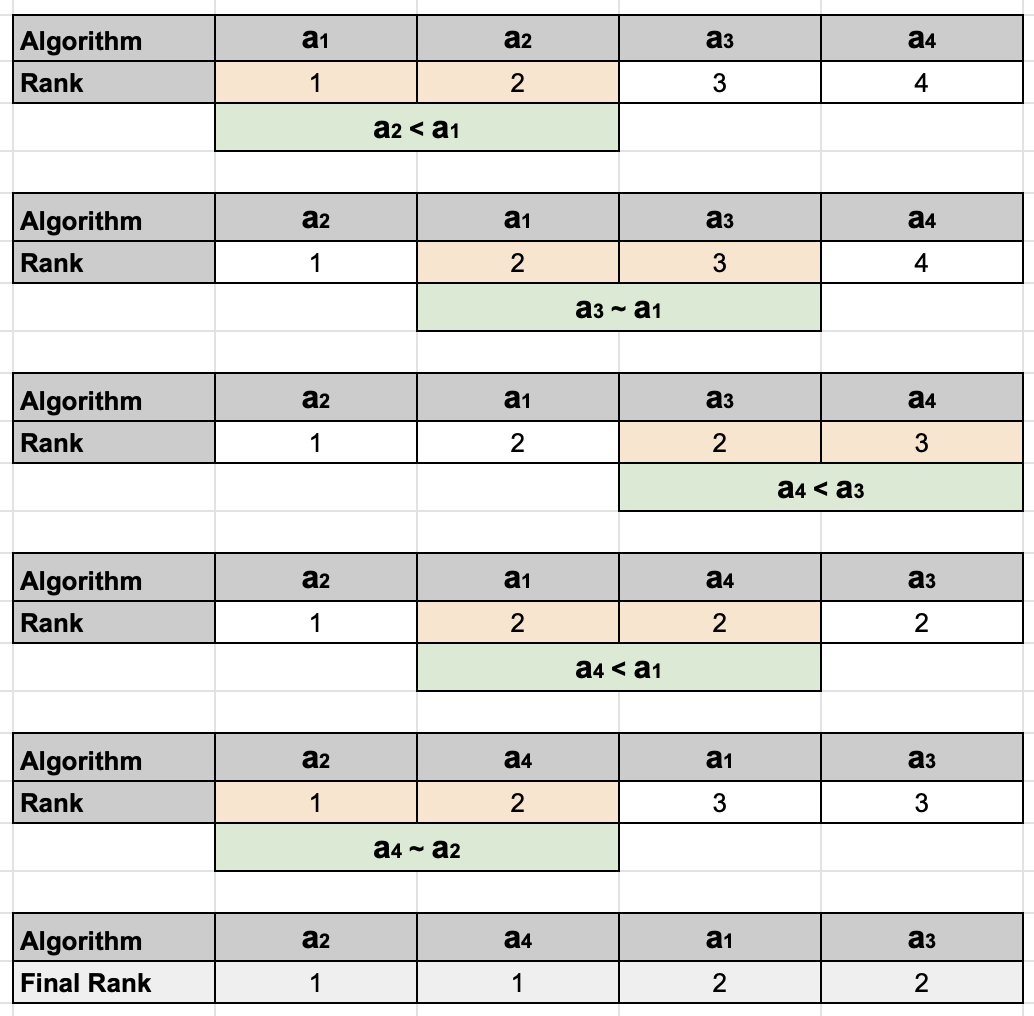
\includegraphics[width=0.5\textwidth]{fig/ranking}
	\caption{Bubble Sort with Compare function}
	\label{fig:sort}
\end{figure}

All the algorithms with rank 1 are assigned to the set of fastest algorithms $\mathcal{F}$. From the above illustration,
$\mathcal{F} \leftarrow \{\mathbf{a_2}, \mathbf{a_4}\}$. Recall that the results of the Compare Function (Procedure \ref{alg:compare}) are not entirely deterministic due to non-transitivity of comparisons. As a consequence, the final ranks obtained by Procedure \ref{alg:sort} are also not entirely deterministic.
For instance, in step 5, algorithm $\mathbf{a_4}$ could be at the threshold  of being better than $\mathbf{a_2}$; that is, if $\mathbf{a_4}$ was
estimated to be better than $\mathbf{a_2}$ once in every two runs of Procedure \ref{alg:sort}, then fifty percent of the times
$\mathbf{a_2}$ would be pushed to rank 2 and would not be assigned to $\mathcal{F}$. To address this, we repeat the Sort function 
$T$ times and in each iteration, all the algorithms that received rank 1 are accumulated in the list $L$. Then, we follow the steps from line 5-9 in Procedure \ref{alg:fa} to compute the relative score. If an
algorithm $\mathbf{a_j}$ was assigned rank 1 in $c$ out of $T$ iterations, then $\mathbf{a_j}$ would appear $c$ times in
the list $L$. Then, the relative confidence (or relative score) for $\mathbf{a_j}$ is $c/T$. 
%Notice that no bootstrapping is done in each of the $T$ iterations (as it was done in Procedure \ref{alg:fa}). The Sort function is repeated only to address the randomness in the final rankings and not to extract more information from the distribution (which is the objective of Bootstrapping that was addressed in the Compare function). 
The modified version of Procedure \ref{alg:fa} is shown in Procedure \ref{alg:f}, which also returns the set of fastest algorithms $\mathcal{F}$ (all the unique occurrences in $L$)
and their corresponding relative scores. Since we are interested only in the fastest algorithms, all the other
candidates that were not assigned rank 1 even once are given a relative score of 0. For the illustration in Figure 1, if $\mathbf{a_4} < \mathbf{a_2}$ in approximately one out of two runs of Sort function, $\mathbf{a_2}$ would get a relative score of 0.5 and $\mathbf{a_4}$ would get 1.0.  $\mathbf{a_1}$ and $\mathbf{a_3}$ would be given relative scores 0.


\begin{algorithm}
	\caption{ Get$\mathcal{F}$$(\mathcal{A})$ }
	\label{alg:f}
	\hspace*{\algorithmicindent} \textbf{Input: } $ \mathbf{a_1},\mathbf{a_2} ,..., \mathbf{a_p}\in \mathcal{A}$ \\
	\hspace*{\algorithmicindent} \textbf{Output: } $ (f_1,c_1), (f_2, c_2), ..., (f_q,c_q) \in \mathcal{F} \times C  $
	\begin{algorithmic}[1] 
		\State $L, C \leftarrow [ \quad ]$ \Comment{Initialize empty lists}
		\For{i = 1, ..., $T$}
		\State $\mathcal{S}, R \leftarrow Sort(\mathcal{A})$
		\State $\tilde{\mathcal{F}} \leftarrow [\mathbf{s}_j | r_j == 1 ]$ \Comment{all algorithms with rank 1}
		\State append($\tilde{\mathcal{F}}, L $)
		\EndFor
		\State $\mathcal{F} \leftarrow $ unique elements in $L$ \Comment{$ q = |\mathcal{F}|$}
		\For{$ i$ in  $f_1,f_2,...,f_q \in \mathcal{F}$}
		\State $c \leftarrow$ number of occurances of $i$ in $L$ 
		\State append($c/T$, $C$)
		\EndFor
		\State return $(\mathcal{F} \times C)$
              \end{algorithmic}
%              \p{same comments apply. Do not use L.append, loops with "for i", syntax, ...}
\end{algorithm}

\section{Experiments}
\label{sec:exp}

For our experiments, we consider the solution algorithms generated by the Linnea framework~\cite{barthels2019linnea}. For a given linear algebra expression with fixed matrix sizes, Linnea generates a family of algorithms in Julia language\cite{julia}.  The distributions of 50 time measurements\footnote{We use the measurement strategy described in Sec. \ref{sec:torel}. The measurements were taken on a dual  socket Intel Xeon E5-2680 v3 with 12 cores each and clock speed of 2.2 GHz running CentOS 7.7. Julia version 1.3 was linked against Intel MKL implementation of BLAS and LAPACK (MKL 2019 initial release).} of four equivalent algorithms (Refer Appendix A for pseudocode) $\mathbf{a}_0, \mathbf{a}_1, \mathbf{a}_2, \mathbf{a}_3 \in \mathbb{R}^{50}$ for the ordinary least square problem  $(X^TX)^{-1}X^{T}y$ is shown in Figure \ref{fig:d}. The measurements were taken under two different settings - in the first setting, the number of threads were fixed to 24; in the second setting, the number of threads for each (of 50) repetition of an algorithm was randomly chosen between 20 and 24. In Figure \ref{fig:d}, the distribution of $\mathbf{a}_0$ is compared against the distributions of other algorithms.  The distributions of $\mathbf{a}_0, \mathbf{a}_1, \mathbf{a}_2$ are largely overlapping; they all perform the same number of floating point operations but differ in the order in which they evaluate matrix operations. Despite similar FLOP counts, the order of computations can still affect the execution time due to cache influence between sequence of calls within the algorithm\cite{peise2014cache}. However, for the sake of validating our methodology, we chose an example where similar FLOP counts result in nearly identical distributions. Algorithm $\mathbf{a}_3$ does twice the number of FLOPs than rest of the algorithms and hence noticeable difference in the distribution is observed.
\begin{figure}
	\centering
	\begin{subfigure}[b]{0.5\textwidth}
		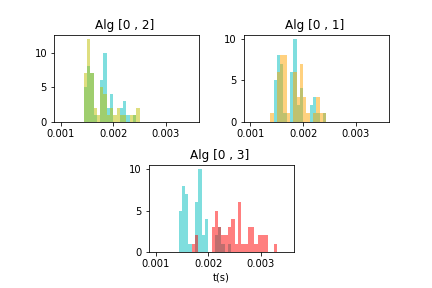
\includegraphics[width=1\linewidth]{fig/f_noise}
		\caption{Setting 1 : Number of threads is set to 24}
		\label{fig:Ng1}
	\end{subfigure}
	
	\begin{subfigure}[b]{0.5\textwidth}
		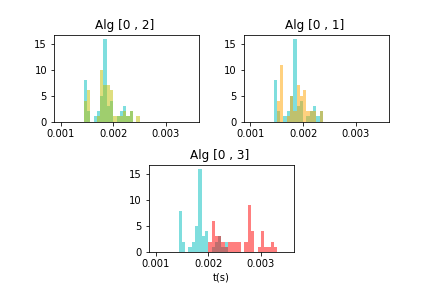
\includegraphics[width=1\linewidth]{fig/f}
		\caption{Setting 2 : Threads are randomly chosen between 20 - 24}
		\label{fig:Ng2} 
	\end{subfigure}
	\caption{Fifty measurements of algorithms 1,2,3 compared against algorithm 0.  Algorithm 0: Blue;  Algorithm 1: Orange; Algorithm 2: Yellow; Algorithm 3: Red.}
	\label{fig:d}
\end{figure}

Recall that the relative scores indicate the chance of an algorithm to be assigned to the set of fast algorithms $\mathcal{F}$. Looking at the distributions, one would naturally expect high scores for $\mathbf{a}_0, \mathbf{a}_1$ and $\mathbf{a}_2$. The assignments made to $\mathcal{F}$ are said to be robust or consistent or reproducible when they not largely influenced by operation setting or when the number of measurements are decreased (from 50).

\subsection{Robustness to Operation settings}

In the introduction, we argued that rankings that are based exclusively on a single number such as minimum or mean execution time to quantify performance would lead to inconsistency when the measurements are reproduced. Table \ref{tab:2} shows the distribution statistics of the algorithms $\mathbf{a}_0, \mathbf{a}_1, \mathbf{a}_2, \mathbf{a}_3$ for the two different settings described earlier. For setting 1,  when the minimum execution time is considered, it can be seen that the best algorithm is $\mathbf{a}_1$. However, when one considers the mean execution time, $\mathbf{a}_1$ is distinctly behind $\mathbf{a}_0$ and $\mathbf{a}_2$. Furthermore, when the measurements are reproduced under setting 2,  both minimum and mean estimates of $\mathbf{a}_1$ lag behind $\mathbf{a}_0$ and $\mathbf{a}_2$. Hence, it is not clear if $\mathbf{a}_1$ can be assigned to $\mathcal{F}$.
\begin{table}[h!]
	\begin{center}
		\renewcommand{\arraystretch}{1.2}
		\begin{tabular}{@{}r rrr c rrr@{}}
			\toprule
			& \multicolumn{3}{c}{Setting 1 (ms)} & & \multicolumn{3}{c}{Setting 2 (ms)} \\
			\cmidrule{2-4} \cmidrule{6-8}
			& min & mean & std && min & mean & std \\
			\midrule
			{$\mathbf{a}_0$ \hfill }& 1.46  & 1.76  & 0.24  && 1.47  & 1.83  & 0.24  \\
			{$\mathbf{a}_1$ } & 1.44  & 1.82   & 0.25  && 1.51  & 1.91   & 0.44  \\
			{$\mathbf{a}_2$ } & 1.46  & 1.75  & 0.28  && 1.45  & 1.85  & 0.24  \\
			{$\mathbf{a}_3$ } & 1.74  & 2.61  & 0.73  && 2.05  & 2.6  & 0.36  \\
			\bottomrule
		\end{tabular}
		\caption{Statistics of the Algorithms}
		\label{tab:2}
	\end{center}
\end{table}

One could argue that, despite inconsistency, the best algorithm that is identified is indeed always one of the fastest algorithms ($\mathbf{a}_0$ or $\mathbf{a}_1$ or $\mathbf{a}_2$). But most often in practice, the best algorithm has to be identified without executing them; for which realistic performance models are needed. Such performance models are usually trained and evaluated against certain ground truth; in our example, the distributions of $\mathbf{a}_0$, $\mathbf{a}_1$, $\mathbf{a}_2$ are indeed nearly identical and it is essential to know the true chances that every algorithm have in order to be assigned to $\mathcal{F}$. To this end, the consistency of performance estimate is important. Furthermore, practical use-cases of identifying not one, but all the fast algorithms are described in Section \ref{sec:app}. 
 
In section \ref{sec:torel}, we then introduced the simple bootstrapping method in Procedure \ref{alg:fa} and argued that it does not take into account the uncertainty in measurement data and therefore the test for significant difference is necessary, in which one algorithm is evaluated to be faster than the other only when there is enough evidence. We then modified Procedure \ref{alg:fa} by incorporating the test for significant difference using the three way Compare function (Procedure \ref{alg:compare}), which is used to sort and rank algorithms into equivalence classes in Procedure \ref{alg:sort}. 
 
In Procedure \ref{alg:compare}, when $M = 1$, the three-way Compare function falls back to a regular comparison with
outcomes $< , >$; as a consequence, the Get$\mathcal{F}$ function (Procedure \ref{alg:f}) reduces to the basic bootstrapping method
described in section \ref{sec:torel}: Procedure \ref{alg:fa}.
%In order to understand the differences in
%relative scores obtained by Procedure \ref{alg:fa} and Procedure \ref{alg:f}, we consider the instance of ordinary least
%square problem with four solution algorithms (as generated by Linnea), each measured fifty times\footnote{The
%  repetitions of each algorithm were not measured consecutively but randomly sandwiched between other algorithms. \p{you
%    explained this, didn't you?} This was done to ensure that the measurements were linearly independent. i.e., unbiased
%  from system noise.}. The algorithms were measured on a \p{ .... } run with 24 threads.
%\p{indicate processor, operating system, and libraries used.}
%In an attempt  to check the invariance (robustness) of relative scores to system noise, the experiments were repeated by
%randomly switching between 20 to 24 threads. \p{this is not clear -- what does ``randomly switching'' mean? you are
%  probably saying that you gathered data for both 20 and 24 threads, but compared them separately} 
Table \ref{tab:1} shows the relative scores obtained by Procedure \ref{alg:fa} ($M=1$  and $threshold$ not applicable) and Procedure
\ref{alg:f} (for different values of $threshold$ with $M=30$).
% \p{Maybe it would be a good idea to repeat the meaning of
%  these scores}
%The experiments were also repeated by randomly switching between 20 to 24 threads to simulate system noise.
% The distributions of the algorithms in comparison with Algorithm 0  are shown in Figure \ref{fig:d}. 
 %Significant overlap can be observed between algorithms 0,1 and 2. 


 		% \begin{tabular}{c|ccc|ccc|}
 		% 	\cline{2-7}
 		% 	& \multicolumn{3}{|c|}{Without Noise} &  \multicolumn{3}{|c|}{With Noise} \\
 		% 	\cline{2-7}
 		% 	& Alg 0 & Alg 1 & Alg 2 & Alg 0 & Alg 1 & Alg 2 \\
 		% 	\hline
 		% 	\multicolumn{1}{ |c| }{M=1, thresh=N/A}  & 0.45 &0.11 &0.44 & 0.53 & 0.07 & 0.40 \\
 		% 	\hline
 		% 	\multicolumn{1}{ |c| }{M=30, thresh=0.50} & 0.53 &0.0 &0.47 & 0.76 & 0.0 & 0.24 \\
 		% 	\hline
 		% 	\multicolumn{1}{ |c| }{M=30, thresh=0.80} & 0.96 &0.73 &0.90 & 0.97 & 0.12 & 0.95\\
 		% 	\hline
 		% 	\multicolumn{1}{ |c| }{M=30, thresh=0.85}& 0.97 &0.89 &0.94 & 0.95 & 0.22 & 0.93 \\
 		% 	\hline
 		% 	\multicolumn{1}{ |c| }{M=30, thresh=0.90} & 0.99 &0.97 &0.99 & 0.95 & 0.66 & 0.90\\
 		% 	\hline
 		% 	\multicolumn{1}{ |c| }{M=30, thresh=0.95}& 1.0 &0.99 &0.99 & 0.97 & 0.88 & 0.97 \\
 		% 	\hline
 		% \end{tabular}



%\p{for all tables, please use tabbing and this next one as a template}
\begin{table}[h!]
  \begin{center}
    \renewcommand{\arraystretch}{1.2}
    \begin{tabular}{@{}r rrr c rrr@{}}
      \toprule
      & \multicolumn{3}{c}{Setting 1} & & \multicolumn{3}{c}{Setting 2} \\
      \cmidrule{2-4} \cmidrule{6-8}
                       & $\mathbf{a}_0$ & $\mathbf{a}_1$  & $\mathbf{a}_2$  && $\mathbf{a}_0$  & $\mathbf{a}_1$  & $\mathbf{a}_2$  \\
      \midrule
      {M=1, \hfill thr=N/A}
                       & 0.45  & 0.11  & 0.44  && 0.53  & 0.07  & 0.40  \\
      {M=30, thr=0.50} & 0.53  & 0.0   & 0.47  && 0.76  & 0.0   & 0.24  \\
      {M=30, thr=0.80} & 0.96  & 0.73  & 0.90  && 0.97  & 0.12  & 0.95  \\
      {M=30, thr=0.85} & 0.97  & 0.89  & 0.94  && 0.95  & 0.22  & 0.93  \\
      {M=30, thr=0.90} & 0.99  & 0.97  & 0.99  && 0.95  & 0.66  & 0.90  \\
      {M=30, thr=0.95} & 1.0   & 0.99  & 0.99  && 0.97  & 0.88  & 0.97  \\
      \bottomrule
    \end{tabular}
    \caption{$T$ = 500, $K$ = 10}
    \label{tab:1}
  \end{center}
\end{table}

For $M=1$, $\mathbf{a}_0$, $\mathbf{a}_1$ and $\mathbf{a}_2$ were assigned to  $\mathcal{F}$ and $\mathbf{a}_1$ received a low relative score in both the settings. Therefore, based on the analysis from $N=50$ time measurements $\mathbf{a}_1$ lagged slightly behind $\mathbf{a}_0$ and $\mathbf{a}_2$. However, 50 measurements are still only a snap shot of the true distribution, which is not available. Therefore, the test for significant
difference is performed and the result of two comparisons is considered equivalent ($\sim$) if there is not enough evidence
that one algorithm dominates the other. The tolerance level up to which two algorithms should be considered equivalent
is controlled by adjusting the $threshold$ parameter in the Compare function. When $threshold=0.5$, the tolerance level is 0 and the outcome $\sim$ in the Compare function is still impossible. When the relative scores are computed with the setting  $M=30$ and $threshold=0.5$, $\mathbf{a}_0$ obtained a score 0 and was strictly not assigned to $\mathcal{F}$.  When $threshold$ is increased, the conditions for one algorithm to be ranked better than the other in Procedure \ref{alg:sort} becomes stricter and as a result, it becomes difficult for $\mathbf{a}_0$ and $\mathbf{a}_2$ to be ranked better than $\mathbf{a}_1$. Therefore, as $threshold$ increased, the relative score of $\mathbf{a}_1$ became higher (see Table \ref{tab:1}), which meant it was assigned with rank 1 more frequently across different repetitions of the  Sort function in Procedure \ref{alg:f}. $\mathbf{a}_3$ still obtained relative score 0; because, its difference from other distributions are noticeable.

%in Fig.~\ref{fig:d}, the
%histogram of Algorithm 0 is compared  against that of Algorithms 1, 2, 3. In spite of the significant overlap observed
%between Algorithms 0 and 1, the latter receives a lower relative score and \p{``and''? what are you pointing out here?
%  Maybe you want to put a . or ; and continue with ``furthermore''}
%the actual mean of Algorithm 1 is also distinctly greater than that of Algorithms 0 and 2 (see Table
%\ref{tab:2}). However the minimum execution time of Algorithm 1 (from the experiment without noise) is smaller than that
%of other algorithms thereby pointing to a contradicting result. This example clearly illustrates that depending
%exclusively on a single summary statistic does not lead to reliable comparisons.
%\p{can you say ``... illustrates that rankings that are based exclusively on ... do not lead to ...''. However, what do
%  we mean by ``reliable comparisons''? and then again, what is the problem with it? I understand the logic, but I do not
%  see any dramatically wrong decision here. A good algorithm might not be in F but another one is (or vice versa), so what?}
 %Moreover, what we have is just a snap-shot of the true distrution and the sample statistics are also just an approximation. 
%Therefore, it is recommended to test for significant differences between the distributions in comparison. 
 %Therefore, the  Whether one wants to consider both these algorithms as equivalent or distinct can be controlled by the threshold.
%Although the histogram comparison between Algorithms 0 and 1 show a more significant overlap in Figure \ref{fig:Ng2} than in Figure \ref{fig:Ng2}

%\begin{table}[h!]
%\begin{center}
%\begin{tabular}{c|ccc|ccc|}
%	\cline{2-7}
%	& \multicolumn{3}{|c|}{Without Noise (ms)} &  \multicolumn{3}{|c|}{With Noise (ms)} \\
%	\cline{2-7}
%	& min & mean & std & min  &mean & std  \\
%	\hline
%	\multicolumn{1}{ |c| }{ Alg 0} & 1.46 & 1.76 & 0.24 & 1.47 & 1.83 & 0.24 \\
%	\hline
%	 \multicolumn{1}{ |c| }{ Alg 1}& 1.44 & 1.82 & 0.25 & 1.51 & 1.91 & 0.44 \\
%	\hline
%	 \multicolumn{1}{ |c| }{ Alg 2}& 1.46 & 1.75 & 0.28 & 1.45 & 1.85 & 0.24 \\
%	\hline
%	\multicolumn{1}{ |c| }{ Alg 3}& 1.74 & 2.61 & 0.73 & 2.05 & 2.6 & 0.36 \\
%	\hline
%\end{tabular}
%	\caption{Statistics of the Algorithms}
%\label{tab:2}
%\end{center}
%\end{table}


%
%In order to extract more information from the available measurements, we set $M=30$ and $threshold =0.5$, which \p{what
%  does ``which'' refer to? I would put s . snd explain: ``with/in this setup, ...''} still uses only the two-way
%comparison in Procedure \ref{alg:compare}, but now the pair-wise comparisons with the minimum statistic is bootstrapped
%before sorting. By doing this,  Algorithm 1 gets a relative score 0 and is strictly not assigned to $\mathcal{F}$ (see
%Table \ref{tab:1}, second row). However, the measurements in Fig.~\ref{fig:d} are just snapshots of the true
%distribution, so an element of uncertainty remains. Therefore, it  is important to perform the test for significant
%difference, by which the result of two comparisons is considered equivalent ($\sim$) if there is not enough evidence
%that one algorithm dominates the other. The tolerance level up to which two algorithms should be considered equivalent
%is controlled by adjusting the $threshold$ parameter in the Compare function. When $threshold$ is increased, the
%conditions for one algorithm to be ranked better than the other in Procedure \ref{alg:sort} become stricter. For
%instance, a threshold value of 0.9 implies that in order for one algorithm to be ranked better than another it would
%have to 
%perform better in at least 9 runs out 10. As a consequence, it becomes difficult for algorithms 0 and 2 to be ranked
%better than algorithm 1 and they all end up clustered with same rank. From Table \ref{tab:1}, it can be seen that as $threshold$ is increased, the relative score of Algorithm 1 becomes higher, which means it is assigned with rank 1 more frequently across different repetitions of the  Sort function in Procedure \ref{alg:f}. Algorithm 3 still gets relative score 0; because, its difference from other distributions are noticeable.

The "tolerance" level is also impacted by the parameter $K$ in Procedure \ref{alg:compare}, which is the number of measurements sampled in each of the $M$ bootstrap iteration. In every iteration of comparing two algorithms $(\mathbf{a_i}, \mathbf{a_j})$, the minimum execution time $(e_i,e_j)$ of the samples ($\mathbf{\tilde{a}_i} \subset \mathbf{a_i}$, $\mathbf{\tilde{a}_j} \subset \mathbf{a_j}$) are computed. As $K \to N (=50)$, the minimum of the samples $(\mathbf{\tilde{a}_i},\mathbf{\tilde{a}_j)}$ would approximate the minimum of the distributions $(\mathbf{a_i}, \mathbf{a_j})$. As a consequence, when $K=50$, the evaluation of $e_i \le e_j$ in the Compare function becomes deterministic and $\sim$ would become an impossible outcome. For Setting 1 in Table \ref{tab:2}, $\mathbf{a}_1$ recorded the least execution time; therefore, as $K \to 50$, the relative score of $\mathbf{a}_1$ approaches 1.0, while the scores of $\mathbf{a}_0$ and $\mathbf{a}_2$ approach 0 (see Figure \ref{fig:k}). 
\begin{figure}[h!]
	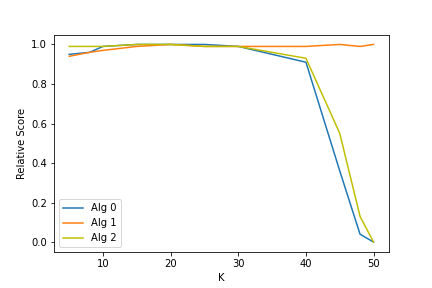
\includegraphics[width=0.5\textwidth]{fig/k}
	\caption{Relative Score vs $K$ \\ $T$=500, $M$=30, $threshold$=0.9}
	\label{fig:k}     
\end{figure}
Thus, higher values of $K$ invalidates the advantages of bootstrapping and  the rankings start depending more and more exclusively on a single statistic. It is ideal to have $K$ randomly chosen from a set of values (say $K \in [5,10]$).
%\begin{figure}
%	\begin{subfigure}[b][0.5\textwidth]
%		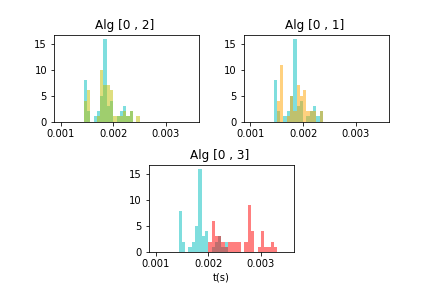
\includegraphics[width=1\linewidth]{fig/f}
%		%\caption{Bubble Sort with Compare function}
%	\end{subfigure}
%	\begin{subfigure}[b][0.5\textwidth]
%		\includegraphics[width=1\linewidth]{fig/f_a}
%		%\caption{Bubble Sort with Compare function}
%	\end{subfigure}
%\end{figure}
\ar{Aravind got here}
\subsection{Robustness to number of measurements}

We evaluate the consistency or robustness of assignments made to $\mathcal{F}$ when the number of measurements $N$ of each algorithm is decreased. Let $\mathcal{F}_{N}$ be the set of fastest algorithms identified with $N$ measurements of each algorithm. As $N$ is decreased, we report the average precision and recall (explained later in this section) of $\mathcal{F}_N $ with respect to $\mathcal{F}_{50}$ in Table \ref{tab:3} for linear algebra expressions from 25 application examples in \cite{barthels2019linnea}.

We consider the solutions to be less robust when the precision is low. Consider the following instance where $\mathcal{F}_{50} : \{0,2\}$ and $\mathcal{F}_{20} : \{0,1,2,3,4\}$. When $N$ is decreased, there is less and less evidence of one algorithm dominating the other in the Compare function and the outcome $\sim$ becomes more and more likely; as a consequence, more algorithms get clustered with rank 1. We assume that $\mathcal{F}_{50}$ is the closer to the true solution than $\mathcal{F}_{N<50}$. When $\mathcal{F}_{20}$ is compared against $\mathcal{F}_{50}$, the set $\mathcal{F}_{20}$ has  $\{0,2\}$ as true positives ($TP$), $\{1,3,4\}$  as false positives ($FP$) and there are no false negatives ($FN$). Therefore, the precision\footnote{precision = $TP/(TP+FP)$} is 0.4 and recall\footnote{recall = $TP/(TP+FN)$} is 1.0. Such a case of low precision but high recall occurs when $M=1$ (see Table \ref{tab:3}) and this could be misleading; although all the fastest algorithms are identified at a lower sample size (resulting in a high recall score), the solution is cluttered with false positives (thereby making it less robust). But for the instance when $\mathcal{F}_{20} : \{2\}$ that has one false negative $\{0\}$ and no false positives, the precision is 1.0 and the recall is 0.5. Although not all the fastest algorithms are identified (resulting in a lower recall score), the identified algorithms are precise (thereby making the solution more robust).
%In practise, for every linear algebra expression $x$ with fixed matrix sizes (or operand sizes) $o$,  Linnea[ref] generates many equivalent algorithms (sometimes over hundreds) and populates $\mathcal{A}(x,o)$. That is, every time the operand sizes are changed, all the algorithms in $\mathcal{A}(x,o)$ should be measured $N$ times in order to be ranked. Therefore, it would be useful if  reliable estimates can be obtained with smaller sample sizes. For expressions from 25 application examples in [linnea], Table ?? shows the variations in precision and recall of the identified set of fastest algorithms $\mathcal{F}(o,x)$  as the number of measurements $N$ is decreased. 
%\begin{table}[h!]
%	\begin{center}
%		\renewcommand{\arraystretch}{1.2}
%		\begin{tabular}{c|cc|cc|cc|cc|}
%			\cline{2-9}
%			& \multicolumn{6}{|c|}{M = 30} &  \multicolumn{2}{|c|}{M=1} \\
%			\cline{2-9}
%			& \multicolumn{2}{|c|}{th=0.9} &  \multicolumn{2}{|c|}{th=0.8} &  \multicolumn{2}{|c|}{th=0.5}&  \multicolumn{2}{|c|}{th=NA} \\
%			\hline
%				\multicolumn{1}{ |c| }{ \textbf{Sample Size}} & \textbf{prc} & \textbf{rec} & \textbf{prc} & \textbf{rec}  &\textbf{prc }& \textbf{rec} & \textbf{prc }& \textbf{rec} \\
%			\hline
%			\multicolumn{1}{ |c| }{ 40} & 0.97 & 0.94 & 0.86 & 0.90 & 0.71 & 0.67 & 0.32 & 0.99 \\
%			\hline
%			\multicolumn{1}{ |c| }{ 35} & 0.95 & 0.94 & 0.91 & 0.87 & 0.78 & 0.65 & 0.31 & 0.99 \\
%			\hline
%			\multicolumn{1}{ |c| }{ 30} & 0.93 & 0.86 & 0.88 & 0.87 & 0.68 & 0.58 & 0.34 & 0.99 \\
%			\hline
%			\multicolumn{1}{ |c| }{ 25} & 0.95 & 0.86 & 0.90 & 0.78 & 0.58 & 0.58 & 0.34 & 0.98 \\
%			\hline
%			\multicolumn{1}{ |c| }{ 20} & 0.97 & 0.80 & 0.93 & 0.75 & 0.50 & 0.38 & 0.36 & 0.95 \\
%			\hline
%			\multicolumn{1}{ |c| }{ 15} & 0.98 & 0.59 & 0.96 & 0.61 & 0.69 & 0.29 & 0.44 & 0.85 \\
%			\hline
%		\end{tabular}
%		\caption{Average Precision and Recall of $\mathcal{F}$ \\T=50, K=10}
%		\label{tab:3}
%	\end{center}
%\end{table}
\begin{table}[h!]
	\begin{center}
		\renewcommand{\arraystretch}{1.2}
		\begin{tabular}{@{}r rr c rr c rr c rr@{}}
			\toprule
			& \multicolumn{8}{c}{$M=30$} & & \multicolumn{2}{c}{$M=1$} \\
			\cmidrule{2-9} \cmidrule{11-12}
			& \multicolumn{2}{c}{thr=0.9} & & \multicolumn{2}{c}{thr=0.8} & & \multicolumn{2}{c}{thr=0.5} & & \multicolumn{2}{c}{thr=NA} \\
			\cmidrule{2-3} \cmidrule{5-6} \cmidrule{8-9} \cmidrule{11-12}
			{$N$} & \textbf{prc} & \textbf{rec} && \textbf{prc} & \textbf{rec} && \textbf{prc} & \textbf{rec} && \textbf{prc} & \textbf{rec} \\
			\midrule
			{40} & 0.97  & 0.94  && 0.86  & 0.90  && 0.71  & 0.67 && 0.32 & 0.99 \\
			{35} & 0.95  & 0.94  && 0.91  & 0.87  && 0.78  & 0.65 && 0.31 & 0.99 \\
			{30} & 0.93  & 0.86  && 0.88  & 0.87  && 0.68  & 0.58 && 0.34 & 0.99 \\
			{25} & 0.95  & 0.86  && 0.90  & 0.78  && 0.58  & 0.58 && 0.34 & 0.98 \\
			{20} & 0.97  & 0.80  && 0.93  & 0.75  && 0.50  & 0.38 && 0.36 & 0.95 \\
			{15} & 0.98  & 0.59  && 0.96  & 0.61  && 0.69  & 0.29 && 0.44 & 0.85 \\
			\bottomrule
		\end{tabular}
		\caption{Average Precision and Recall of $\mathcal{F}$ \\$T$=50, $K$=10}
		\label{tab:3}
	\end{center}
\end{table}
 From Table \ref{tab:3}, it can be seen that the precision improves considerably when $M=30$ even with zero tolerance (i.e., $threshold = 0.5$). Furthermore, the precision improves as $threashold$ increases, but this is partly due to the fact that more algorithms are now assigned with rank 1. For the instance previously discussed, $\mathcal{F}_{50}$ had just two algorithms $\{0,2\}$ at $threshold = 0.5$, but when $threshold = 0.9$ the set now has $ \{0,1,2,3\}$. This is because the conditions for algorithms 0 and 2 to be ranked better than 1 and 3 became stricter. Now the same solution $\mathcal{F}_{20} : \{0,1,2,3,4\}$ that was obtained with $M=1$ will have a higher precision score (0.8). Therefore, improved precision at higher thresholds comes with a cost of having higher tolerance (to allow for same rank even with lesser overlap of distributions) or stricter conditions for one algorithm to be ranked better than the other. 
 
 \section{Why is Relative Performance important?}
 \label{sec:app}
 In the past decade, we have witnessed an increasing number of latency sensitive applications involving intelligent vehicles\cite{connectedvehicles}, real-time video analytics\cite{videoanalytics}, augmented reality\cite{arvr} etc.,  that require costly scientific computations on resource-constrained hardware. Offloading all the computations to a cloud is not a viable solution for such applications because of unacceptable communication latency between the cloud and end devices\cite{surveyMCC} \cite{towardsEdgeComputing}. On the other hand, increasing capabilities of mobile devices enable them to be more suitable for scientific computing\cite{smartPhonesForScientificComputing} \cite{raspberryEdgeComputing}. Consequently, there is a trend of computation offloading\cite{surveyOfComputationalOffloading2013} toward edge computing \cite{edgeComputing2016} \cite{towardsEdgeComputing} \cite{edgeComputing2015}, where significant gains are realized when computations are shifted towards the edge of the network (including the local device)\cite{EdgeComputingQuantifying}. For instance, a proof-of-concept platform that runs face recognition application in \cite{facerecog} shows that the response time is reduced from 900 to 169 ms by moving computation from cloud to the edge. 
% Depending on the distribution of workload among devices, one could come up with myriads of implementation for the same computational problem, each having a significant impact on both latency and energy consumption. Clone cloud in \cite{clonecloud} does on-demand partitioning of workload between mobile and the cloud, and their prototype could reduce 20x running time and energy for the tested application.
 
 Increasing number of such applications in recent times can be attributed to containerization tools like Docker\cite{docker} that ease portability of code without compromising performance\cite{dockerForEdgeComputing} \cite{dockerhpc} and enable the use of same Linux environment across heterogeneous devices. Further more, recent high level programming languages like Julia\cite{julia}, Tensorflow\cite{tensorflow}, PyTorch\cite{pytorch} etc that abstract the calls to linear algebra libraries optimized for different hardware (such as raspberry Pi, GPU), allow developers to write code without worrying about the underlying architecture and yet achieve close to machine performance. While benchmarking suites like \cite{cavbench}\cite{edgeaibench} are used to evaluate performance over the network, it is also important to find out if the single node devices also achieve the required performance. Linear algebra computations, which appear at the heart of most scientific computations can have hundreds of equivalent implementations, each  with different performance footprints\cite{barthels2019linnea} and therefore selection of the right implementation is equally significant.
 
\section{Conclusion and Future Outlook}
\label{sec:con}
We presented a measurement-based approach to identify all equivalently fast algorithms for computing a given linear
algebra expression via relative performance. Linear algebra operations occur at the heart of most mathematical
computations and are one of the major computational bottlenecks, therefore identification of high performance code is essential. For instance, the resilience of a flying drone to atmospheric conditions can be improved if the on-board processor can compute a few extra gradient per second. 
The typical development of linear algebra code involves a lot of trial and error in choosing the best implementation out
of several possible alternatives. In order to automate code development, \p{languages such as ...} and compilers such as
Linnea~\cite{barthels2019linnea} were developed to automatically decompose a mathematical expression into sequences of
library calls. 
The selection of best algorithm can be guided by models that predict relative performance. Therefore, a natural extension to this work would be "Relative Performance modelling", where we aim to automatically predict (or model) the relative scores without having to execute all the algorithms.

\bibliographystyle{IEEEtran}
\bibliography{references}

\clearpage
\section*{Appendix}
\subsection{Equivalents Algorithms for Ordinary Least Square Problem}
\label{sec:appA}
\begin{algorithm}
	\renewcommand{\thealgorithm}{}
	\floatname{algorithm}{Algorithm 0}
	\caption{ Blue }
	\label{alg:a0}
	\textbf{Expression: } $(X^TX)^{-1}X^{T}y \qquad X \in \mathbb{R}^{1000 \times 500} \quad y \in \mathbb{R}^{500}$ 
	\begin{algorithmic}[1] 
		\State $T_1 \leftarrow syrk(X^{T}X)$ \Comment{$T_1^{-1}X^{T}y$}
		\State $LL^{T} \leftarrow $ Cholesky($T_1$) \Comment{$L^{-T}L^{-1}X^{T}y$}
		\State $t_2 = X^{T}y$ \Comment{$L^{-T}L^{-1}t_2$}
		\State $t_2 = L^{-1}t_2$ \Comment{$L^{-T}t_2$}
		\State $z = L^{-T}t_2$
	\end{algorithmic}
\end{algorithm}

In \textbf{Algorithm 1} and \textbf{Algorithm 2}, the order in which computations are evaluated are changed but the FLOP count remains the same as \textbf{Algorithm 0}. Still, the order of computations can affect the execution time due of cache effects between sequence of calls\cite{peise2014cache}.
\begin{algorithm}
	\renewcommand{\thealgorithm}{}
	\floatname{algorithm}{Algorithm 1}
	\caption{ Orange }
	\label{alg:a0}
	\textbf{Expression: } $(X^TX)^{-1}X^{T}y \qquad X \in \mathbb{R}^{1000 \times 500} \quad y \in \mathbb{R}^{500}$ 
	\begin{algorithmic}[1] 
		\State $t_1 = X^{T}y$ \Comment{$(X^{T}X)^{-1}t_1$}
		\State $T_2 \leftarrow syrk(X^{T}X)$ \Comment{$T_2^{-1}t_1$}
		\State $LL^{T} \leftarrow $ Cholesky($T_2$) \Comment{$L^{-T}L^{-1}t_1$}
		\State $t_1 = L^{-1}t_1$ \Comment{$L^{-T}t_1$}
		\State $z = L^{-T}t_1$
	\end{algorithmic}
\end{algorithm}

\begin{algorithm}
	\renewcommand{\thealgorithm}{}
	\floatname{algorithm}{Algorithm 2}
	\caption{ Yellow }
	\label{alg:a0}
	\textbf{Expression: } $(X^TX)^{-1}X^{T}y \qquad X \in \mathbb{R}^{1000 \times 500} \quad y \in \mathbb{R}^{500}$ 
	\begin{algorithmic}[1] 
		\State $T_1 \leftarrow syrk(X^{T}X)$ \Comment{$T_1^{-1}X^{T}y$}
		\State $t_2 = X^{T}y$ \Comment{$T_1^{-1}t_2$}
		\State $LL^{T} \leftarrow $ Cholesky($T_1$) \Comment{$L^{-T}L^{-1}t_2$}
		\State $t_2 = L^{-1}t_2$ \Comment{$L^{-T}t_2$}
		\State $z = L^{-T}t_2$
	\end{algorithmic}
\end{algorithm}

The FLOP count for \textbf{Algorithm 3} is 2x more than the previous algorithms.
\begin{algorithm}
	\renewcommand{\thealgorithm}{}
	\floatname{algorithm}{Algorithm 3}
	\caption{ Red }
	\label{alg:a0}
	\textbf{Expression: } $(X^TX)^{-1}X^{T}y \qquad X \in \mathbb{R}^{1000 \times 500} \quad y \in \mathbb{R}^{500}$ 
	\begin{algorithmic}[1] 
		\State $T_1 \leftarrow gemm(X^{T}X)$ \Comment{$T_1^{-1}X^{T}y$}
		\State $LL^{T} \leftarrow $ Cholesky($T_1$) \Comment{$L^{-T}L^{-1}X^{T}y$}
		\State $t_2 = X^{T}y$ \Comment{$L^{-T}L^{-1}t_2$}
		\State $t_2 = L^{-1}t_2$ \Comment{$L^{-T}t_2$}
		\State $z = L^{-T}t_2$
	\end{algorithmic}

\end{algorithm}
\end{document}

%%% Local Variables:
%%% mode: latex
%%% TeX-master: t
%%% End:
